% Please make sure you insert your
% data according to the instructions in PoSauthmanual.pdf
\documentclass[a4paper,11pt]{article}
\usepackage{pos}
\usepackage{xcolor}
\usepackage{subcaption} % Modern package for subfigures
\usepackage{graphicx}   % Required for inserting images

\usepackag{bbm}
\newcommand{\dd}{\mathrm{d}}
\newcommand{\deint}[2]{\dd^{#1}\;\!\!#2\;}
\newcommand{\br}[1]{\left\langle #1 \right |}
\newcommand{\kt}[1]{\left| #1 \right \rangle}
%
\newcommand\brktt[3]{\left< #1 \right| #2 \left| #3 \right>}
\newcommand{\bkt}[2]{\left \langle #1 |#2 \right \rangle}
\newcommand{\brkt}[2]{\left \langle #1 |#2 \right \rangle}
\newcommand{\eps}{\epsilon}
\newcommand{\cEFT}{$\chi$EFT}
\newcommand{\etal}{\textit{et al.}}
\newcommand{\Li}{\mathrm{Li}}
\newcommand{\LiS}{{}^{6} \mathrm{Li} }
\newcommand{\HeF}{{}^{4} \mathrm{He}}
\newcommand{\HeT}{{}^{3} \mathrm{He}}
\newcommand{\HT}{{}^{2} \mathrm{H}}
\newcommand\bv[1]{\vec{#1}}
\newcommand{\ques}[1]{\color{red}\textit{ #1 }\color{black}}
\newcommand\ddfrac[2]{\frac{\displaystyle #1}{\displaystyle #2}}
\newcommand{\MeV}{\mathrm{MeV}}

\title{Scattering Observables from Few-Body Densities and Application
in Light Nuclei}
%% \ShortTitle{Short Title for header}

\author*[a]{Alexander Long}
\author[a]{Harald Griesshammer}

\affiliation[a]{The George Washington University\\ Washington DC USA}
% \affiliation[a]{Institution,\\
%   Street number, City, Country}

% \affiliation[b]{Department, University,\\
% Street number, City, Country}

\emailAdd{alexlong@gwu.edu}
\emailAdd{hgrie@gwu.edu}

\abstract{
  The dynamics of scattering on light nuclei is well understood, but
  calculation is numerically difficult using standard methods.
  Fortunately using recent developments, the relevant quantities can
  be factored into a product of the $n$-body transition densities and
  the interaction kernel of a chosen probe.
  These  transition densities depend only on the target, and not the
  probe; they are calculated once and stored.
  The kernels depend on only the probe and not the target.
  The calculation of the transition densities becomes numerically
  difficult for $n\ge4$, but we discuss a solution through use of a
  renormalization
  group transformation.
  This technique allows for extending the density transition method to $\HeF$
  and $\LiS$.
  Throughout this work Compton scattering is used as test bed
  but extension to pion-photoproduction is discussed as well.
}

\FullConference{The 11th International Workshop on Chiral Dynamics (CD2024)\\
  26-30 August 2024\\
Ruhr University Bochum, Germany\\}

%% \tableofcontents

\begin{document}
\maketitle

\section{Introduction}
\ques{This can be 10 pages. Anything is red is a question or
  something that needs to be fixed.\\~\\ I am a little unclear on how
  much discussion of effective field theories, and general intro
  information is needed here.
}

The transition density method was pioneered by Griesshammer \etal
\cite{hammer2020}.
An incoming probe striking an $A$ body nucleus may interact with
$1,2...A$ nucleons.
The $n$ nucleons it interacts with we call \textit{active} and $A-n$
it does not we call \textit{spectators}.
The mathematical description of these two parts are completely
separate; the active nucleons contribute to the kernel and spectator
nucleons contribute to the density.
The complete separation of these two parts means if one has access to
$a$ different kernels and $b$ different nucleus descriptions, then
$ab$ different results can be produced.
Figure \ref{fig:onetwobod} provides an example for the case $A=3$.

\begin{figure}[h!]
  \begin{center}
    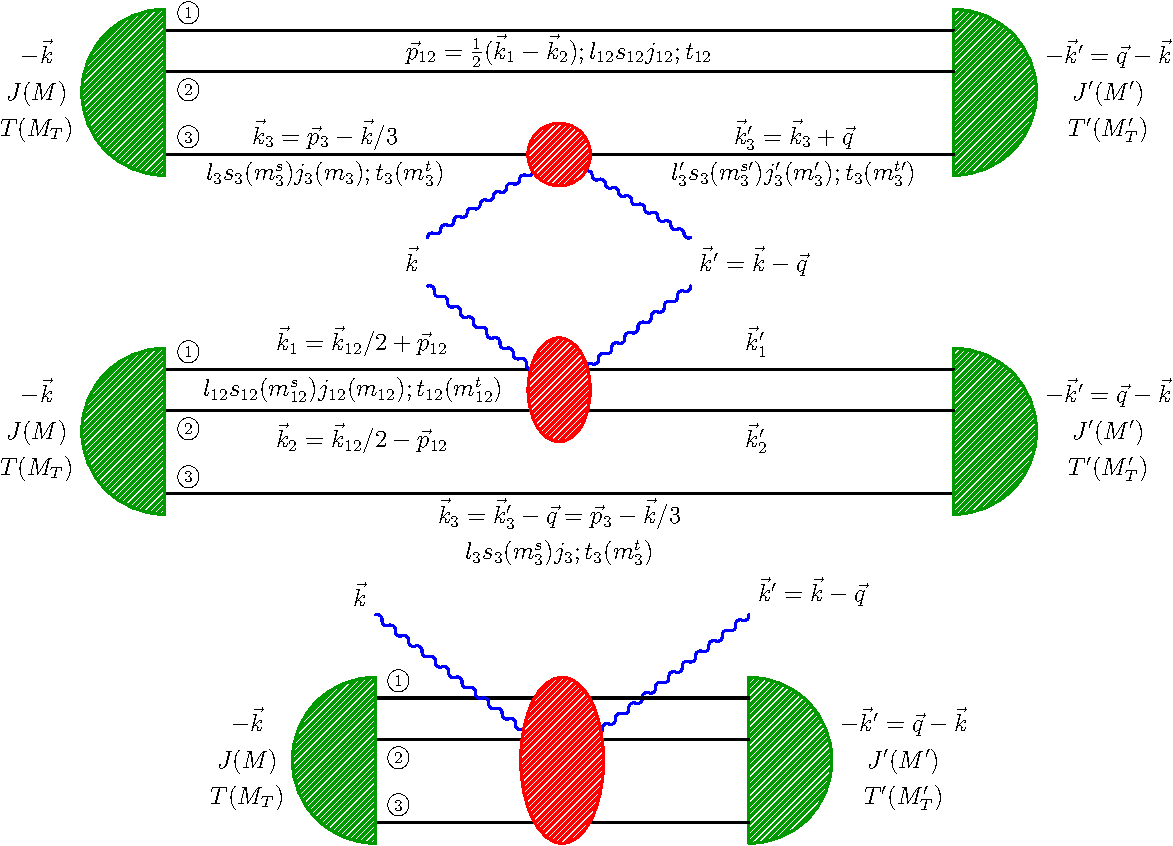
\includegraphics[scale=0.7]{kinematics3He.pdf}
    \caption{Kinematics in the center of mass frame and quantum
      numbers for an $A=3$ system in the case of Compton scattering.
      Generalization to other reactions only changes the kind of
      ingoing/outgoing probe. Top: one-body processes, center: two-body
      processes, bottom: three-body processes. Green represents the
      densities, and red represents the kernels. Griesshammer \etal
    \cite{hammer2020}}
    \label{fig:onetwobod}
  \end{center}
\end{figure}

For scattering off an $A$ body nucleus, the total scattering
amplitude is given by
\begin{align}
  A_{M}^{M^{\prime} }(\bv{k}, \bv{q})&=\binom{A}{1}\left\langle
  M^{\prime}\right|\hat{O}_{3}^{}(\bv{k}, \bv{q})\left|M\right
  \rangle + \binom{A}{2} \left\langle
  M^{\prime}\right|\hat{O}_{12}^{}(\bv{k}, \bv{q}) \left|
  M\right\rangle\nonumber\\
  &+ \binom{A}{3}\left\langle
  M^{\prime}\right|\hat{O}_{123}^{}(\bv{k}, \bv{q})\left|M\right
  \rangle + \binom{A}{4} \left\langle
  M^{\prime}\right|\hat{O}_{1234}^{}(\bv{k}, \bv{q}) \left| M\right\rangle\\
  &+... + \binom{A}{A}\left\langle
  M^{\prime}\right|\hat{O}_{1...A}^{}(\bv{k}, \bv{q})\left|M\right
  \rangle,\nonumber
\end{align}
where $M,M'$ is the spin of the target nucleus, and there are
$\binom{A}{i}$ ways for a probe to hit $i$ nucleons. Fortunately
$\chi$EFT provides a hierarchy of scales which predicts decreasing
contributions for higher order terms for energies greater than $\sim 40 \MeV$.
To this end we use only the first two terms
\begin{equation}
  A_{M}^{M^{\prime} }(\bv{k}, \bv{q})=\binom{A}{1}\left\langle
  M^{\prime}\right|\hat{O}_{3}^{}(\bv{k}, \bv{q})\left|M\right
  \rangle + \binom{A}{2} \left\langle
  M^{\prime}\right|\hat{O}_{12}^{}(\bv{k}, \bv{q}) \left|
  M\right\rangle\nonumber\\
\end{equation}
In practice this is enough for accuracy on the 5\% level.
\section{Kernels and Densities}
The one-body and two-body kernel need to be considered separately.
Their form is completely different, and they require a one and two
body density respectively.
We now write the wave function in the three body system as the
partial-wave decomposition of Jacobi momenta $p_i$ and the relevant
quantum numbers $\alpha$. The wave function in momentum space is given by
\begin{equation}
  \psi_\alpha (p_{12},\, p_3 ) = \bkt{p_{12} p_3 \alpha}{M}.
\end{equation}
The nucleus being described has total angular momentum $J$ and
spin-projection $M$. The momenta are $\bv{p}_{12}= \frac{1}{2}
\left(\bv{k}_1 - \bv{k}_2\right)$ where $ \bv{p}_3 = \bv{k}+
\frac{1}{3} \bv{k}_3 $, and $p_{12} = |\bv{p}_{12}|$ and  $p_{1} =
|\bv{p}_{1}|.$ Recall $\bv{k}_i$ are the individual nucleon momenta,
and $\bv{k}$ is the probe momentum in the CM frame. The quantity
$\alpha$ represents all the quantum numbers of the nucleons inside
the nucleus~\cite{hammer2020}:
\begin{equation}
  |\alpha\rangle=\left|\left[\left(l_{12} s_{12}\right)
  j_{12}\left(l_{3} s_{3}\right) j_{3}\right] J M,\left(t_{12}
  t_{3}\right) T M_{T}\right\rangle,
\end{equation}
where $s$, $l$ and $j$ are the spin, orbital and total angular
momentum respectively. The quantum number $s_3$ simply represent the
spin of nucleon 3, whereas $s_{12}$ represents the total spin of the
1-2 subsystem; the quantities $l_{12}$ and $j_{12}$ combine the 1-2
subsystem similarly. Furthermore, $s_{12}$ and $l_{12}$ combine to
$j_{12}$ and likewise for $l_3$, $s_3$ and $j_3$. Finally $j_{12}$
and $j_3$ combine to the total nucleus spin $J$.
The same combinations are done for $t_{12}$, $t_3$ and $T$, with
isospin projection $M_T$. Here $t_3$ and $t_{12}$ are the isospin of
the nucleon labeled 3 and the 1-2 subsystem respectively, $T$ is the
isospin of the entire nucleus and $M_T$ is the number of protons
minus neutrons over 2.
We now seek to describe the scattering amplitudes.

We restrict ourselves to elastic processes, which simplifies the
following discussion by requiring that the probe does not change the
charge of any of the nucleons.
For the one body density, the \textit{one-body kernel} of the probe
interaction with nucleon 3 is $O_3$. Leaving nucleons $1$ and $2$ as
spectators~\cite{hammer2020},
\begin{align}
  &\left\langle\bv{k}_{3}^{\prime}\left|\left\langle s_{3} m_{3}^{s
  \prime}\left|\left\langle t_{3} m_{3}^{t
  \prime}\left|\hat{O}_{3}(\bv{k}, \bv{q})\right| t_{3}
  m_{3}^{t}\right\rangle\right| s_{3} m_{3}^{s}\right\rangle\right|
  \bv{k}_{3}\right\rangle \nonumber\\
  &\qquad\qquad\qquad \equiv \delta_{m_{3}^{t \prime} m_{3}^{t}}
  \delta^{(3)}\left(\bv{k}_{3}^{\prime}-\bv{k}_{3}-\bv{q}\right)
  O_{3}\left(m_{3}^{s \prime} m_{3}^{s} m_{3}^{t} ; \bv{k}_{3} ;
  \bv{k}, \bv{q}\right),\label{dirac}
\end{align}
where $m_t$ and $m_t'$ are the isospin of the active nucleon before
and after the interaction (recall $m_t= \pm \frac{1}{2}$ is the proton/neutron).
Symbolically, the matrix element $\hat{O}_3$ is:
\begin{align}
  \left\langle M^{\prime}\left|\hat{O}_{3}(\bv{k}, \bv{q})\right|
  M\right\rangle&=\sum_{\alpha \alpha^{\prime}} \int \mathrm{d}
  p_{12} p_{12}^{2} \mathrm{~d} p_{3} p_{3}^{2} \mathrm{~d}
  p_{12}^{\prime} p_{12}^{\prime 2} \mathrm{~d} p_{3}^{\prime}
  p_{3}^{\prime 2}
  \psi_{\alpha^{\prime}}^{\dagger}\left(p_{12}^{\prime}
  p_{3}^{\prime}\right) \psi_{\alpha}\left(p_{12} p_{3}\right)\nonumber \\
  &\times\left\langle p_{12}^{\prime}
  p_{3}^{\prime}\left[\left(l_{12}^{\prime} s_{12}^{\prime}\right)
    j_{12}^{\prime}\left(l_{3}^{\prime} s_{3}\right)
  j_{3}^{\prime}\right] J^{\prime} M^{\prime}\left(t_{12}^{\prime}
  t_{3}\right) T^{\prime} M_{T}\right| \hat{O}_{3}(\bv{k}, \bv{q})
  \label{onebodyExplicit}\\
  &\qquad\qquad\left|p_{12} p_{3}\left[\left(l_{12} s_{12}\right)
  j_{12}\left(l_{3} s_{3}\right) j_{3}\right] J M\left(t_{12}
  t_{3}\right) T M_{T}\right\rangle.\nonumber
\end{align}
The central result is that up to relativistic corrections, this can
be written as:
\begin{align}
  \left\langle M^{\prime}\left|\hat{O}_{3}(\bv{k}, \bv{q})\right|
  M\right\rangle=\sum_{\substack{m_{3}^{s \prime}\,
  m_{3}^{s}\\m_3^t}}\hat{O}_{3}\left(m_{3}^{s \prime} m_{3}^{s},
  m_{3}^{t} ;  \bv{k}, \bv{q}\right) \rho_{m_{3}^{s \prime}
  m_{3}^{s}}^{m_3^{t} M_{T}, M^{\prime} M}(\bv{k}, \bv{q})\label{onebodyOrig}\;.
\end{align}
Here $\rho$, is the \textit{one-body transition density amplitude}
for the nucleus which was discussed previously and can truly be
interpreted as the probability amplitude that nucleon $m_3^t$ absorbs
momentum $\bv{q}$, changes its spin projection from $m_s^3$ to
$m_s^{3'}$ and changes the spin-projection of the nucleus from $M$ to
$M'$. Its operator form is
\begin{equation}
  \rho_{m_{3}^{\prime} m_{3}^{s}}^{m_{3}^{t} M_{T}, M^{\prime}
  M}(\bv{k}, \bv{q})=\left\langle M^{\prime}\right.\left|s_{3}
  m_{3}^{s \prime}, t_{3} m_{3}^{t}\right\rangle
  \mathrm{e}^{\mathrm{i} \frac{2}{3} \bv{q} \cdot
  \bv{r}_{3}}\left\langle s_{3} m_{3}^{s}, t_{3}
  m_{3}^{t}\right|\left. M\right\rangle\label{onebody}.
\end{equation}
The two body case works similarly, and results in
\begin{equation}
  \left\langle M^{\prime}\left|\hat{O}_{12}\right| M\right\rangle =
  \sum_{\alpha_{11}^{\prime}, \alpha_{12}} \int \mathrm{d} p_{12}\:
  p_{12}^{2} \mathrm{~d} p_{12}^{\prime}\: p_{12}^{\prime 2}\;
  O_{12}^{\alpha_{12}^{\prime} \alpha_{12}}\left(p_{12}^{\prime},
  p_{12}\right) \rho_{\alpha_{12}^{\prime} \alpha_{12}}^{M_{T},
  M^{\prime} M}\left(p_{12}^{\prime}, p_{12} ; \bv{q}\right)\label{twobody}\;.
\end{equation}
This two-body density $\rho_{\alpha_{12}^{\prime}
\alpha_{12}}^{M_{T}, M^{\prime} M}$ is of course completely distinct
from the one-body density and has a more involved expression
equivalent to \eqref{onebody}.
This two-body density can also be interpreted as a probability density.
It is dependent on the incoming and outgoing quantum numbers
$\alpha_{12}$ and $\alpha_{12}'$ of the 1-2 system, and also on the
relative momenta of the two nucleons which are integrated over.
As a result, the total file size for the two nucleon densities are on
the order of a few GB per energy and angle, whereas those of the one
nucleon densities are on the order of a few KB.
Importantly, $\rho$ can be computed generically from a nuclear
potential, such as the chiral SMS potential 
without reference to the kernel $\hat{O}_3$ or $\hat{O}_{12}$ \cite{Reinert2018}.
\ques{Maybe this is too much detail.}

\section{SRG Transform}
Previous work using the transition density method has looked at $\HeT$ and $\HeF$ but to extend this $\LiS$ involves many body iterations which are much more complicated, and numerically expensive to compute \cite{hammer2020, hammer4He}. 
To this end a similarity renormalization group (SRG) transformation is used \cite{SRG}.
In general a nuclear potential, such as the chiral SMS potential does not fall off quickly for high momentum meaning we would have to extend the cutoff much further than we would like which in turn increases computation cost.
The SRG transform is a unitary transformation that allows us to shovel all the dependence into the low momentum region making calculation for $A=6$ possible.
The SRG transformation can be thought of as a local averaging or smoothing out of the potential, resulting in decreased "resolution" has the SRG is applied.
\begin{figure}[h]
    \centering
    \begin{subfigure}{0.45\textwidth}
        \centering
        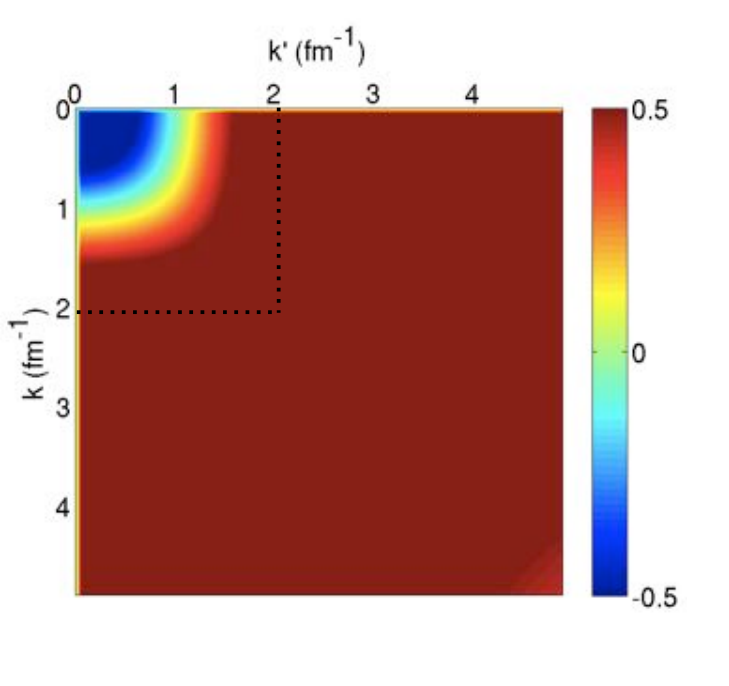
\includegraphics[width=\linewidth]{HighRes.png}
        \caption{High Resolution (bare, unevolved potential) }
        \label{fig:highres}
    \end{subfigure}
    \hfill
    \begin{subfigure}{0.45\textwidth}
        \centering
        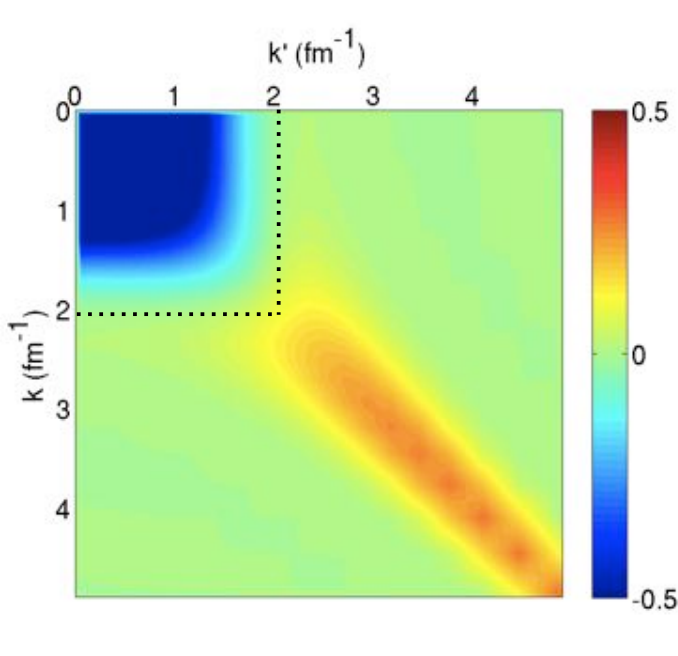
\includegraphics[width=\linewidth]{LowRes.png}
        \caption{Low Resolution (evolved)}
        \label{fig:lowres}
    \end{subfigure}
    \caption{Nuclear potentials $V(k,k')$. Figures from Kai Hebeler: ``Chiral Effective Field Theory and Nuclear Forces:
overview and applications'' presentation at TALENT school at MITP 2022}
    \label{fig:SRGtransform}
\end{figure}
In the unevolved, high resolution figure \ref{fig:highres} one can see the potential does not go to zero quickly whereas once the transformation is applied in figure \ref{fig:lowres} it does. As a result a cutoff can be made at $k,k'=2 \mathrm{fm}^{-1}$ without losing much accuracy. In the example above, if the unevolved potential had to be consider up to $k,k'=5$, this means an efficiency gain of $(5/2)^2=6.25$.

However, this creates another problem; the SRG transform creates a change in physical meaning of the momenta free variables.
To understand this, let us first consider an example the reader is certainly more familiar with - a Fourier transformation which changes a potential from position to momentum space.

\begin{equation}
    V(\vec{r},\vec{r}\,')= \br{r'} V \kt{r}=
                          \int \dd^3p\, \dd^3p' \brkt{r'}{p'} \br{p'}V\kt{p} \brkt{p}{r}\\
                          =V(\vec{p},\vec{p}\,')
\end{equation}
After the transform our free variables have different physical meaning. In fact, any unitary transform, also transforms the coordinates.
\begin{align}
    \br{p'}V\kt{p} &= \br{p'} \mathbbm{1} V \mathbbm{1} \kt{p}\nonumber\\
                   &= \br{p'} U^\dag U V U^\dag U \kt{p}\nonumber\\
                   &= \left(\br{p'} U^\dag\right)\;\left( U V U^\dag\right)\;\left( U \kt{p}\right)\\
                   &= \br{\widetilde{p}\,'} V_{eff} \kt{\widetilde{p}}=V_{eff}(\widetilde{p},\widetilde{p}\,')\nonumber
\end{align}
in the case of the SRG transform this has significant consequences.
\section{Uncertainty}
Integrations blah blah... Convergence and cutoffs blah blah...

\section{Conclusion}
\begin{thebibliography}{99}
  \bibitem{hammer2020}
  H. W. Grie{\ss}hammer, J. A. McGovern, A. Nogga, and D. R.
  Phillips, ``Scattering Observables from One- and Two-body
  Densities: Formalism and Application to $\gamma^3$ Scattering,''
  \textit{Few-Body Systems}, vol. 61, no. 4, Nov. 2020. DOI:
  \href{https://doi.org/10.1007/s00601-020-01578-w}{10.1007/s00601-020-01578-w}.

  \bibitem{Reinert2018}
  P. Reinert, H. Krebs, and E. Epelbaum, ``Semilocal momentum-space
  regularized chiral two-nucleon potentials up to fifth order,''
  \textit{The European Physical Journal A}, vol. 54, no. 5, May 2018.
  DOI:
  \href{http://dx.doi.org/10.1140/epja/i2018-12516-4}{10.1140/epja/i2018-12516-4}.
  \bibitem{hammer4He}
  H. W. Griesshammer, J. Liao, J. A. McGovern, A. Nogga, and D. R.
  Phillips, ``Compton Scattering on 4He with Nuclear One- and
  Two-Body Densities,'' arXiv preprint, 2024. Available:
  \href{https://arxiv.org/abs/2401.16995}{arXiv:2401.16995}.

  \bibitem{SRG}
S. Szpigel and R. J. Perry, ``The Similarity Renormalization Group,'' arXiv preprint, 2000. Available: \href{https://arxiv.org/abs/hep-ph/0009071}{arXiv:hep-ph/0009071}.
\end{thebibliography}

\end{document}
